\chapter{Algebraic Diagrammatic Construction (ADC)}

The \acl{ADC} is a Green's function approach, which is a method for the
calculation of ionization
energies and electron affinities.
Its advantage is the ability to determine the desired ionization energies
without explicit calculation of the initial and final states, but instead
obtaining their energy differences directly.
Moreover, this approach is size-consistent and is hence
suitable for the description of larger systems. \cite{Mertins96_1}

Originally, the Green's function was formulated in the Dyson ansatz and
determined using perturbation theory. This way both the ionization and the
electron affinity part had to be included in the description. In the non-Dyson
scheme those two are separable and hence, the dimension of the problem is reduced
when one is interested in either the $N+1$ (electron affinity)
or the $N-1$ (ionization energy) part \cite{Schirmer98}.

\begin{equation}
 G_{pq}(\omega) = G^+_{pq}(\omega) + G^-_{pq}(\omega)
\end{equation}

The ionization part $\mathbf{G^-}(\omega)$ is a function of the energy
$\omega$ and is transposed to give
$\tilde{G}^-_{pq}(\omega) = G^-_{qp}(\omega)$. From this, the compact 
and orthogonal matrix
form can be deduced

\begin{equation}\label{matrixspec}
\mathbf{\tilde{G}}^-(\omega) = \mathbf{x}^\dagger
                               (\omega\mathds{1}-\mathbf{\Omega})^{-1}\mathbf{x}
\end{equation}

where $\mathbf{x}$ are the spectroscopic amplitudes and $\mathbf{\Omega}$ is
the diagonal matrix of energy eigenvalues.
This diagonal representation was reformulated using Goldstone diagrams
into the non-diagonal expression

\begin{equation}\label{isradc}
\mathbf{\tilde{G}}(\omega) = \mathbf{f}^\dagger(\omega\mathds{1}-\mathbf{M})^{-1}\mathbf{f}
\end{equation}

where $\mathbf{M}$ denotes the \ac{ADC} matrix and $\mathbf{f}$ denotes
the effective transition moments.
Later it was found that this transformation could alternatively be
derived by inserting a set of so-called \emph{intermediate states}
\cite{Schirmer91}.
These are formally constructed from \ac{CES}, which are constructed
using the same kind of excitation operators as in an \ac{CI} expansion.
In contrast to the \ac{CI} approach, the \ac{CES}
are constructed from these operators
acting on the exact and therefore correlated groundstate rather than the
Hartree Fock ground state. These \ac{CES} are then
grouped into excitation classes
and these classes are orthogonalized with respect to each other. Afterwards,  
the states within each class are orthogonalized \cite{Mertins96_1}.

Equation (\ref{isradc}) can be solved by
considering the eigenvalue problem
\begin{equation}\label{adcewp}
\mathbf{M} \mathbf{Y} = \mathbf{Y}\mathbf{\Omega} \quad\text{with } \mathbf{Y}^\dagger\mathbf{Y}=\mathbf{1}
\end{equation}

The spectroscopic amplitudes $\mathbf{x}$ can then be obtained from the
effective transition moments $\mathbf{f}$ as

\begin{equation}
 \mathbf{x} = \mathbf{Y}^\dagger \mathbf{f}
\end{equation}

To this point, the approach is exact.
For the actual construction of the \ac{ADC} matrix $\mathbf{M}$ and the
effective transitions moments $\mathbf{f}$, $\mathbf{M}$ and $\mathbf{f}$
are expanded into different orders of perturbations based on the
M{\o}ller-Plesset partitioned Hamiltonian.

\begin{eqnarray}
\mathbf{M} &=& \mathbf{M}^{(0)} + \mathbf{M}^{(1)} + \mathbf{M}^{(2)} + \cdots\label{stf}\\
\mathbf{f} &=& \mathbf{f}^{(0)} + \mathbf{f}^{(1)} + \mathbf{f}^{(2)} + \cdots\label{stf}
\end{eqnarray}

From this, different orders of perturbation theory of the Hamiltonian can be
constructed successively. Hereby, the truncation after the $n$-th order leads
to ADC($n$). The contributions to the different classes for different
orders of \ac{ADC} are shown
in Figure \ref{figure:adcmat_pgf} \cite{Trofimov05}.

\begin{figure}[h]
  \centering
  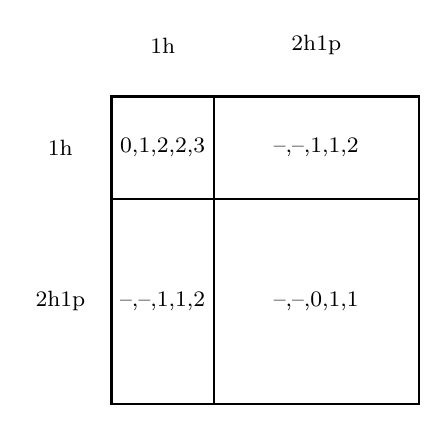
\begin{tikzpicture}[scale=1.3]
    \footnotesize
    %\draw [help lines] (-1,0) grid (23,5);
    \draw [thick] (0,0) rectangle (3,3);
    \draw [thick] (0,2) rectangle (1,3) node [midway] {0,1,2,2,3};
    \draw [thick] (1,0) rectangle (3,2) node [midway] {--,--,0,1,1};
    \draw [thick] (0,0) rectangle (1,2) node [midway] {--,--,1,1,2};
    \draw [thick] (1,2) rectangle (3,3) node [midway] {--,--,1,1,2};
    \node (1h1) at (0.5,3.5) {1h};
    \node (1h2) at (-0.5,2.5) {1h};
    \node (2h1) at (2.0,3.5) {2h1p};
    \node (2h2) at (-0.5,1.0) {2h1p};

\end{tikzpicture}

  \caption{Schematic illustration of an \ac{ADC}($n$) matrix for different orders
           of perturbation for $n=0,1,2,2x,3$. In the illustration, the respective
           highest order contribution is shown for the different blocks.
           Hence, ADC(2x) is an extended ADC(2) including first
           order contributions to the satellite block.}
  \label{figure:adcmat_pgf}
\end{figure}

The matrix elements of ADC(2x) are explicitly given by
\begin{itemize}
 \item 1h/1h (1h block):
   \begin{align}
    M_{kk'}^{(0)} &= \varepsilon_k \delta_{kk'} \\
    M_{kk'}^{(1)} &= 0 \\
    M_{kk'}^{(2)} &= -\frac12 \sum\limits_{abl} V_{ab[kl]} V_{k'l[ab]} %\times
                     \frac{\varepsilon_a+\varepsilon_b-\varepsilon_l
                       -\frac12 \varepsilon_k-\frac12 \varepsilon_{k'}}
                     {(\varepsilon_a+\varepsilon_b-\varepsilon_k-\varepsilon_l)
                      (\varepsilon_a+\varepsilon_b-\varepsilon_{k'}-\varepsilon_l)}
   \end{align}
 \item 1h/2h1p (coupling block):
   \begin{equation}
    M_{j,akl}^{(1)} = V_{kl[aj]}
   \end{equation}
 \item 2h1p/2h1p (satellite block):
   \begin{align}
    M_{akl,a'k'l'}^{(0)} &= (-\varepsilon_a+\varepsilon_k+\varepsilon_l)
                             \, \delta_{aa'}\delta_{kk'}\delta_{ll'} \\
    M_{akl,a'k'l'}^{(1)} &= -\delta_{aa'} V_{k'l'[kl]} + \delta_{kk'} V_{al'[a'l]}
                            +\delta_{ll'} V_{ak'[a'k]} - (k \leftrightarrow l)
   \end{align}
\end{itemize}

Here, $\varepsilon_r$ denotes the $r$-th Hartree Fock orbital energy.
The occupied states are labelled
by $i,j,k,\dots$ and the unoccupied states are labelled by $a,b,c,\dots$. The
two-electron integrals for any combination of occupied and unoccupied orbitals
labelled by $p,q,r,s$ read as
\begin{equation}
 V_{pqrs} = \braket{\varphi_p(1)\varphi_q(2) |V(1,2)| \varphi_r(1)\varphi_s(2)}
\end{equation}

and $V_{pq[rs]} = V_{pqrs} - V_{pqsr}$.

